\documentclass[free]{flammie}

\usepackage{linguex}

\usepackage{tcolorbox}

\definecolor{corpusframe}{RGB}{66,66,66}
\definecolor{corpusback}{RGB}{222,222,222}
\definecolor{chatgptframe}{RGB}{66,0,0}
\definecolor{chatgptback}{RGB}{222,33,33}
\definecolor{gramdivvunframe}{RGB}{0,66,0}
\definecolor{gramdivvunback}{RGB}{33,222,33}
\definecolor{divvungreen}{RGB}{105,220,66}
\definecolor{samired}{RGB}{198,53,31}

\usepackage[normalem]{ulem}

\newcommand\gecfail{\bgroup\markoverwith%
{\textcolor{blue}{\lower3.5pt\hbox{\sixly{}\char58}}}\ULon}

\usepackage[inline]{enumitem}


\title{Exploring Limitations and Risks of LLM-Based Grammatical Error Correction
for Indigenous Languages}


\author{Flammie A Pirinen \\
  Divvun \\
  UiT Norgga árktalaš universitehta \\
  Tromsø, Norway \\
  \texttt{flammie.pirinen@uit.no} \\\and%
  Linda Wiechetek \\
  Divvun \\
  UiT Norgga árktalaš universitehta \\
  Tromsø, Norway \\
  \texttt{linda.wiechetek@uit.no} \\}


\begin{document}
\maketitle
\begin{abstract}
    Rule-based grammatical error correction has long been seen as the most
    effective way to create user-friendly end-user systems for grammatical error
    correction (GEC). However, in the recent years the large language models and
    generative AI systems based on that technology have been progressed fast to
    challenge the traditional GEC approach. In this article we show which
    possibilities and limitations this approach bears for Indigenous languages
    that have more limited digital presence in the large language model data and
    a different literacy background than English. We show experiments in North
    Sámi, an Indigenous language of Northern Europe.
\end{abstract}

\section{Introduction}

\textit{Grammatical error correction} (GEC) is a crucial for supporting writers
in their writing process, especially new writers and those who do a large
workload in production and translation of administrative texts, educational
material, news articles, fiction.

For writers of Indigenous languages proofing tools have an even higher
significance which is due to literacy in these languages. Indigenous and
minority languages that compete with an official majority language typically
stand much stronger orally than written, and competent speakers are not
necessarily competent in writing to the same degree as in speech. However, a
feeling of competence is an important factor in text production, and writers
typically feel more confident when they can verify grammar and spelling.  An
increase in high-quality text production (representative of the language we want
as an output) again is an important factor in developing large language models.
In other words, we need a sufficient amount of the type of language we want to
be produced as an input to the models, and in order to build a text corpus, we
need someone to writing skills and motivate native speakers to write.  Behind
that is usually the work of highly motivated native language experts who
actively push forward a language revitalization
process~\cite{olthuis2013revitalising}.  As a part of this process, language
technology can provide the necessary tools like spell- and grammarcheckers.

Up until late it has been obvious that linguistically demanding tasks like
grammatical error correction require a component of expert-built, rule-steered
grammar, not only to be accurate enough, but also to have the legitimacy of an
expert controlling the language norms and ongoing standardisation.  However, in
the few recent years it has raised into a question if more data-driven
approaches can also work for this problem.  In this article we perform some
experiments to find out to which extent this is plausible and what kind of
limitations there are.

The \textit{research question} we solve in this article is to evaluate how
efficient the contemporary large language models are in the actual task of
grammatical error correction---specifically in endangered language context with
North Sámi as example study. We set to find out the effort needed to
use them and develop existing systems. We also consider how much work it might
take to fix problems in the large language models versus rule-based models when
it comes to, e.g.\ bad suggestions and mistakes in the error detection (i.e.\
false positives).  Regardless of the paradigm, the improvement of the system is
driven by developers with language skills or developers with linguists
co-operating, a resource that is very sparse. Another dimension is how
time-critical the system is; a high quality GEC is a time critical resource for
Indigenous language maintenance and revitalisation in digital era and leaving a
low quality or disfunctional GEC with a promise of potential better version in
the future is unacceptable.

\section{Background}

Grammatical error correction system for Indigenous languages in the Sámi region
have existed for over a decade.~\cite{Wiechetek2012constraint} These systems use
rule-based approaches to natural language processing: Finite-State
Morphology~\cite{beesley2003finite} for modelling lexica and morphology and
Constraint Grammar~\cite{karlsson1990constraint} for modelling linguistic
grammars including syntax. Rule-based approaches have historically been
considered as an ideal fit for grammatical error correction, since it directly
concerns writing grammatical rules. In a rule-based approach it is possible to
target exact grammatical phenomena and also provide user feedback precise to the
situation: ``if there is a first singular personal pronoun and verb in third
singular form, mark an error and tell user about the mismatch, suggest using
first singular form of the verb instead'' would be a typical grammatical order
of action in a GEC tool build on rule-based natural language processing system.
Historically, statistical and data-driven approaches have been limited to
flagging unlikely word-forms and suggesting more likely forms, without
addressing complex grammatical constructions or the logical error that leads to
the error and eventually helps the writer to understand what has gone wrong.
The missing link between error and cause in these approaches deprives the user
of understanding their mistakes and improving their grammar. However, it has
been suggested that the LLM-based approaches may be able to overcome this
limitation, and, at least the most popular chatbot-driven user interface to
large language models does indeed generate explanations alongside corrections
when requested. Inspired by these innovations we decided to test the current
capabilities of large language models and compare them to the rule-based
approach.

The open source LanguageTool~\cite{naber2003rule} and the closed-source browser
plugin / webapp Grammarly~\cite{alikaniotis2019unreasonable} are two of the most
widely used GEC tools. On top of that popular office applications like Google
Docs provide writers aids, which seem to mainly focus on spelling errors, but
may contain grammatical error correction features as well. We have not found
suitable scientific documentation of these to give a fair comparison.

\subsection{Languages and literacy}

We are experimenting with North Sámi, an Indigenous and low-resource language of
Northern Europe. With approx. 20,000 speakers according to
Ethnologue~\cite{ethnologue} it is the biggest of the 9 Sámi languages. It is
spoken in Norway, Finland and Sweden and competing with the three national
majority languages Norwegian, Finnish and Swedish as (nearly) all speakers of
North Sámi are bilingual.  While Finnish and Sámi are related (Finno-Ugric)
languages, Sámi and Norwegian/Swedish are on opposite branches of the language
tree. Bilingualism and loss of language domains are the cause of a higher
frequency of grammatical errors among North Sámi writers. On the other hand, the
widespread use of technologies requires us to express ourselves in writing in
all domains. If the Sámi languages are to have a digital future, written Sámi
needs to be strengthened and correction tools need to be available for
everybody.


\subsection{Risks related to quality of GEC}

When we think of spell- and grammar checkers as tools that somewhat enforce a
language standard in the same way as a teacher and educational books, we rely on
a high level of knowledge/accuracy from these language authorities. Proofing
tools that do not comply with these high standards will eventually have a
negative effect on their user communities. In the case of Indigenous user
communitites this effect can be even stronger if proofing tools are used in the
absence of daily language arenas and language experts.  Related research in the
field of spell-checking and correction for L2 learners in schools
suggests~\cite{hogstrom2024not} that there are patterns of usage of automatic
language correcting tools that can be detrimental to the end-users.  Some of the
problems of this sort can be avoided by ensuring the quality of GEC.\


One trend of data-driven language technology products for (minority) languages
has been providing inferior products to the existing rule-based ones, promising
that they will be improved eventually. However, for example as it is in the case
of spellchecking for Finnish, in the past 10 or so years, the so-called
autocomplete set of spelling checkers have not improved to be able to handle
rare morphologically complex word-forms at all, which is a clear downgrade from
earlier rule-based spellcheckers. For example, a recent version of gboard
Finnish keyboard for android does not think \textit{ovikoodit} `door codes,
i.e.\ keycodes for a door' is a word and marks it as an error, while it is a
normal and quite lexicalised compound already. On another example, it
erroneously suggest that the correct \textit{suukoistamme} `about our kisses' is
replaced with the more likely \textit{puukoistamme} `about our knives', which
apparently exists in the training data.  In order for future GEC to be useful
and not destructive, problems leading to this sort of downgrades ought to be
fixed before pushing them to end users.

\section{Methods}

We are using two existing systems out of the box for comparison: one rule-based
and one based on the large language model technology. We use the systems as
black boxes, without rewriting the existing rules of the rule-based systems and
without finetuning or re-training the large language model. In the rule-based
system, we use command-line tooling to get suggestions for the grammatical error
corrections with explanations and with the LLM we use the available chat
interface to get corrections and explanations. The LLM is prompted in English
and advised to do Grammatical Error Correction.

Here are two pictures showing the end-user experience of grammar checking with
the two systems as it is now, see \textit{ChatGPT} in Figure~\ref{fig:chatgpt}
and \textit{GramDivvun} in Figure~\ref{fig:gramdivvun}.\ \textit{ChatGPT}
helpfully provides a translation of the sentence with its error correcting
explanations.  It translates \textit{jáhkkán} with the gerund \textit{waiting}
instead of past participle \textit{thought} and by that introduces two errors--
one semantic and one syntactic. The correction \textit{jáhkán} is not a gerund
as promised, but a first person singular. The list of flaws for this short
sentence goes on and on.\  \textit{Guorosnaga} does not mean \textit{suddenly},
but \textit{empty-handed} and the spelling correction to \textit{guorusnaga} is
incorrect.\ \textit{[G]ii livččii} does not mean \textit{who was}, but
\textit{who would have (thought)}.\  \textit{[J]a dál diekkár} means \textit{and
now that}, which is entirely correct and should not be corrected to \textit{ja
dál diehtá}.


\begin{figure*}
    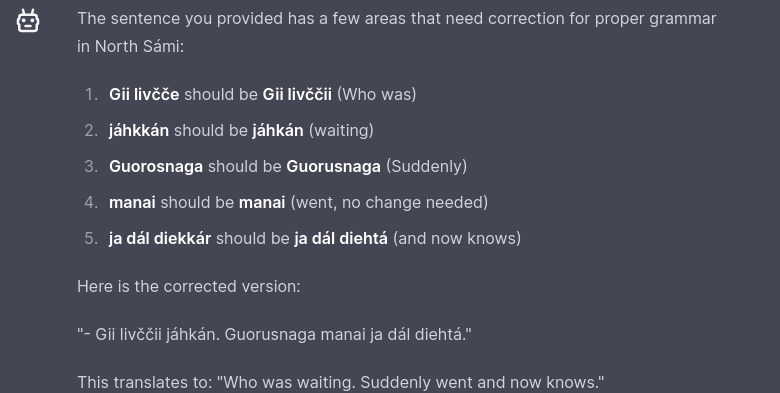
\includegraphics[width=\textwidth]{chatgpt-gramcheck.png}
    \caption{ChatGPT correcting a sentence in North Sámi.\label{fig:chatgpt}}
\end{figure*}

\begin{figure*}
    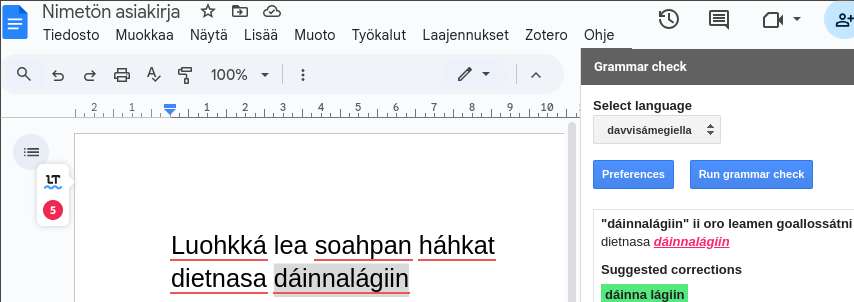
\includegraphics[width=\textwidth]{gramdivvun.png}
    \caption{\textit{GramDivvun} in Google Docs correcting a
    sentence with default red lines for corrections of English
    language\label{fig:gramdivvun}}
\end{figure*}


We have gathered an error corpus by harvesting sentences with several types of
grammatical errors, where we focused on
\begin{enumerate*}
    \item frequent errors in the error corpus
and
    \item errors of different main types and complexity.
\end{enumerate*}
The main grammatical error
types are categorized in the error corpus are lexical
errors (misuse and non-idiomatic use of a word), real-word errors (forms that are
likely caused by a typo, but result in existing words), morpho-syntactic errors
(errors that have a syntactic impact, where the difference between error and
correction can be described by means of morphology), syntactic errors (errors
that have a syntactic impact, where the difference between error and correction
requires adding/taking away or moving one or several word forms). In addition,
the error data contains punctuation and style errors. We have not evaluated the
punctuation and style errors in this article.


\begin{figure}
%    \begin{tcolorbox}[colframe=black, colback=white]
    \begin{verbatim}
Mus {eai}£{verb,fin,sg3prs,
pl3prs,kongr|ii}
leat dihtor dahje TV.
    \end{verbatim}
%    \end{tcolorbox}
    \caption{Example of marked up error in the hand-annotated
    corpus.\label{markup}}
\end{figure}

The Figure~\ref{markup} shows the raw corpus data for a morpho-syntactic error.
The third person plural verb \textit{eai} does not agree with the singular
subject \textit{dihtor} `computer', cf.\ ex.~\ref{TV}.

%\begin{tcolorbox}[colframe=corpusframe, colback=corpusback, arc=2mm]
\exg. Mus \textbf{*eai} leat dihtor dahje TV.\label{TV}\\
I\textsc{.loc} \textsc{neg.3pl} be\textsc{.conneg} computer\textsc{.nom.sg} or
TV\textsc{.nom.sg}\\
`I don't have a computer or a TV'.

%\end{tcolorbox}

In this investigation, we focused only on the two categories of morpho-syntactic
and syntactic errors, specifically the error types represented in
Table~\ref{errortypes}. Since we are using real-world texts as test data, some
of the sentences do contain further error types; this is common and unavoidable
in the realistic use cases for Indigenous corpora and GEC.\


\begin{table}
    \small
    \centering
    \begin{tabular}{lr}
        \toprule
        Error type &  Instances \\
        \midrule
        Adjective inflection errors & 6 \\
        Global agreement errors (subject-verb) & 7 \\
        Nominal case errors & 8 \\
        Compound errors (2$>$1) & 6 \\
        \bottomrule
    \end{tabular}
    \caption{Morpho-syntactic and syntactic error types\label{errortypes}}
\end{table}



\section{Results and discussion}

To evaluate the grammatical error correction systems, we have collected and
hand-annotated 101 sentences, some of which are error-free and
some which have one or more errors. We have done both quantitative and
qualitative analysis of the error corrections performed by both
\textit{GramDivvun} and \textit{ChatGPT}.

To get a rough idea of the quality, we measured the precision and recall using
the usual formulas, on a per error basis, counting a correction as a true
positive only when the detected error and the correction are exactly the correct
substrings, true negative, when no errors were expected and none were marked,
false positive, when system marked a non-error substring as an error and false
negative, when system did not flag an error substring, or also when all
corrections were incorrect. The statistics resulting are shown in the
figure~\ref{fig:f-scores}. We included an $F_{0.5}$ score to underscore our
preference for high precision over high recall.

\begin{table}
% \small
    \centering
    \begin{tabular}{lrrr}
        \toprule
        System & Precision & Recall & $F_{0.5}$ \\
        \midrule
        GramDivvun & 58~\% & 60~\% &  0.58 \\
        ChatGPT & 17~\% & 13~\%  & 0.16 \\
        \bottomrule
    \end{tabular}
    \caption{Precision, recall and $F_{0.5}$ scores of the systems
    we tested.\label{fig:f-scores}}
\end{table}


We have performed a linguistic error analysis on both correction sets and
summarised the results in the following Subsection~\ref{subsec:error-analysis}.

\subsection{Error Analysis}\label{subsec:error-analysis}

We first analyse common North Sámi grammatical error types linguistically
keeping in mind the probable cause of the error from the end-user perspective.
We then show how both GEC tools do the grammatical error analysis
(successfully/unsuccessfully) and summarise our findings.  The source texts are
presented in examples~\ref{luohkka},~\ref{hijiri},~\ref{livcce},~\ref{ovdalgo},
and~\ref{arbejuohku} followed by \textit{ChatGPT}'s corrections in
examples~\ref{luohkka-gpt},~\ref{hijiri-gpt},~\ref{livcce-gpt},~\ref{ovdalgo-gpt},
and~\ref{arbejuohku-gpt}, and
\textit{GramDivvun}'s~\ref{luohkka-gd},~\ref{hijiri-gd},~\ref{livcce-gd},~\ref{ovdalgo-gd},
and~\ref{arbejuohku-gd} respectively.

Example~\ref{luohkka} has a compound error in \textit{dáinnalágiin} `in this
way'. It is perceived as a semantic unit, therefore many people write it as one
word. However, the official spelling requires it to be two words.  In
example~\ref{hijiri} there aren't any grammatical errors.  Example~\ref{livcce}
has a common verb error in \textit{livčče}, which is due to dialectal forms that
are not used in the written standard. In order to satisfy subject-verb agreement
third person plural \textit{livčče} should be third person singular
\textit{livččii}.  Example~\ref{ovdalgo} has another subject-verb agreement
error. The first person plural verb \textit{guorahallat} should be third person
plural \textit{guorahallet} in agreement with the nominal subject in plural. For
uneven-syllable verbs, first and third person plural forms in present tense are
homonymous. However, for uneven syllable verbs that is not the case.  In
example~\ref{arbejuohku}, there is an adjective error. In North Sámi, adjective forms
differ with regard to their position in the sentence. In this sentence it is
used before a noun, i.e.\ attributively. However, the form used here is
predicative \textit{álkis}. The correct form is \textit{álkes}.



A common type of error with \textit{ChatGPT} is that it comes up with non-words
as a corrections, as in example~\ref{luohkka-gpt}.

%\begin{tcolorbox}[colframe=corpusframe, colback=corpusback, arc=2mm]
    \exg. Luohkká lea soahpan háhkat dietnasa \gecfail{dáinnalágiin}\label{luohkka}\\
class have\textsc{.prs.3sg} agree\textsc{.ptcp} provide income in.this.way\\
`The class has agreed to provide the income this way'.

%\end{tcolorbox}


%\begin{tcolorbox}[colframe=chatgptframe, colback=chatgptback, arc=2mm]
    \ex. Luohkká lea soahpan háhkat dietnasa \gecfail{dáidnalaččat}\label{luohkka-gpt}

%\end{tcolorbox}

%\begin{tcolorbox}[colframe=gramdivvunframe, colback=divvungreen!90!black, arc=2mm]
    \ex. Luohkká lea soahpan háhkat dietnasa \gecfail{dáinna
    lágiin}\label{luohkka-gd}

%\end{tcolorbox}

In this example \textit{ChatGPT} came up with the nonsense word
\textit{dáidnalaččat}.\  \textit{GramDivvun}, on the other hand, splits the
compound as it should.


In the following example~\ref{hijiri} \textit{ChatGPT} corrects the predicative
adjective form \textit{boaris} to adjective \textit{boares}, where it should not
be corrected.\  \textit{GramDivvun}, correctly, does not give us this false
correction. However, it does not recognize the foreign name \textit{Hijiri} and
corrects it to \textit{Hiiri}.

%\begin{tcolorbox}[colframe=corpusframe, colback=corpusback, arc=2mm]
\exg. Sin namat leat Jola ja Hijiri. Jola lea gávcci jagi boaris. Hijiri lea logi jagi boaris.\\
    They\textsc{.gen.pl} name\textsc{.pl.nom} be\textsc{.prs.3pl} Jola and
    Hijiri. Jola be\textsc{.prs.3sg} eight\textsc{.sgg.gen} year\textsc{.sg.gen}
    old. Hijiri be\textsc{.prs.3sg} ten\textsc{.sg.gen} year\textsc{.sg.gen} old.\\
`Their names are Jola and Hijiri. Jola is eight years old. Hijiri is ten years
    old'.\label{hijiri}

%\end{tcolorbox}

%\begin{tcolorbox}[colframe=chatgptframe, colback=samired, arc=2mm]
    \ex. \gecfail{Sii} namat leat Jola ja Hijiri. Jola lea gávcci jagi
    \gecfail{boares}. Hijiri lea logi jagi \gecfail{boares}.\label{hijiri-gpt}

%\end{tcolorbox}

%\begin{tcolorbox}[colframe=gramdivvunframe, colback=divvungreen!90!black, arc=2mm]
    \ex. Sin namat leat Jola ja \gecfail{Hiiri}. Jola lea gávcci jagi boaris.
    Hiiri lea logi jagi boaris.\label{hijiri-gd}

%\end{tcolorbox}

In the following example~\ref{livcce} \textit{ChatGPT} corrects the third person
verbal form \textit{livčče} to third person singular \textit{livččii} correctly.
However, it introduces two realword errors which were not there beforehand,
\textit{jáhkkán}$>$\textit{jáhkán} (changing past participle to first person
singular present tense and the demonstrative pronoun), \textit{diekkár} to a
similar sounding third person singular verb \textit{diehtá}.\
\textit{GramDivvun} corrects the agreement error correctly, and does not
introduce any false positives.

%\begin{tcolorbox}[colframe=corpusframe, colback=corpusback, arc=2mm]
    \exg.  Gii \gecfail{livčče} jáhkkán. Guorosnaga manai ja dál
diekkár.\label{livcce}\\
Who be\textsc{.cond.3pl} think\textsc{.ptcp}. Empty-handed go\textsc{.past.3sg} and then that.\\
`Who would have thought. S/he went there empty-handed and then that'.

%\end{tcolorbox}

%\begin{tcolorbox}[colframe=chatgptframe, colback=chatgptback, arc=2mm]
    \ex. Gii \gecfail{livččii} \gecfail{jáhkán}.\ \gecfail{Guorusnaga} manai ja
    dál \gecfail{diehtá}.\label{livcce-gpt}

%\end{tcolorbox}

%\begin{tcolorbox}[colframe=gramdivvunframe, colback=divvungreen!90!black, arc=2mm]
    \ex. Gii \gecfail{livččii} jáhkkán. Guorosnaga manai ja dál
    diekkár.\label{livcce-gd}

%\end{tcolorbox}

In example~\ref{ovdalgo}, \textit{ChatGPT} erroneously introduces a new lexeme,
i.e.\ \textit{mánáid} `children', instead of \textit{mánusiid} `manuscript'.
Neither \textit{ChatGPT}, nor \textit{GramDivvun} manage to correct the
subject-verb agreement error and change first person plural \textit{guorahallat}
to third person plural \textit{guorahallet} in agreement with the plural subject
\textit{konsuleanttat}.

%\begin{tcolorbox}[colframe=corpusframe, colback=corpusback, arc=2mm]
\exg. Ovdalgo ášši joavdá dán muddui, de konsuleanttat \gecfail{*guorahallat} mánusiid.\\ %}£{verb,fin,pl3prs,pl1prs,kongr|guorahallet}
Before thing move\textsc{.prs.3sg} this way, then consultants deal.with\textsc{.prs.1pl} manuscript\textsc{.acc.pl}\\
`Before the matter goes this way, the consultants deal with the
    manuscripts'.\label{ovdalgo}

%\end{tcolorbox}

%\begin{tcolorbox}[colframe=black, colback=chatgptback, arc=2mm]
    \ex. Ovdalgo ášši \gecfail{joavddá} dán muddui, de konsuleanttat guorahallat
    \gecfail{mánáid}.\label{ovdalgo-gpt}

%\end{tcolorbox}

%\begin{tcolorbox}[colframe=black, colback=divvungreen!90!black, arc=2mm]
\ex. Ovdalgo ášši joavdá dán muddui, de konsuleanttat guorahallat
    mánusiid.\label{ovdalgo-gd}

%\end{tcolorbox}


%\begin{tcolorbox}[colframe=corpusframe, colback=corpusback, arc=2mm]
    \exg. Árbejuohku lei duššiid dihte  ma\ng\ng{}onan, ja gárvvisin jurd­dašuvvon
     \gecfail{álkis} kuohku lei šaddan váddáseabbon. \\
Árbejuohku lei duššiid dihte  maŋŋonan, ja gárvvisin jurd­dašuvvon
     álkis kuohku lei šaddan váddáseabbon. \\
     `The inheritance settlement had been delayed due to trivial matters, and
     the planned simple settlement had become more
     complicated'.\label{arbejuohku}

%\end{tcolorbox}

%\begin{tcolorbox}[colframe=black, colback=samired, arc=2mm]
    \ex. Árbejuohku lei \gecfail{dušše} dihte
     maŋŋonan, ja gárvvisin jurd­dašuvvon álkis
    juohku lei šaddan váddáseappot.\label{arbejuohku-gpt}

%\end{tcolorbox}

%\begin{tcolorbox}[colframe=black, colback=divvungreen!90!black, arc=2mm]
    \ex. Árbejuohku lei duššiid dihte
    ma\ng\ng{}onan, ja gárvvisin jurd­dašuvvon \gecfail{álkes}
    juohku lei šaddan váddáseabbon.\label{arbejuohku-gd}

%\end{tcolorbox}

\textit{GramDivvun} corrects the adjective error \textit{álkis} to attributive
\textit{álkes}.\@ \textit{ChatGpt}, on the other hand, firstly, does not find the
adjective error and secondly, corrects several forms that are correct in the
original sentence, \textit{duššiid} `nonsense' to \textit{dušše} `only' and
\textit{váddáseabbon} to \textit{váddáseappot}.  Both, \textit{ChatGpt} and
\textit{GramDivvun} find the spelling error \textit{kuohku} and correct it to
\textit{juohku}.




\subsection{Discussion}

As an overall conclusion of \textit{ChatGPT}'s performance, the overwhelming
problem is the false positive rate, which can be rather bothersome for end-users
and, more importantly, contradicts the authorative nature of a spell- and
grammarchecker in language expertise. The rule-based grammar checker, which
performs significantly better in our experiment, can have issues with recall at
the expense of not alerting the user with false positives. An open question for
the LLM-based approach is, what kind of effort it would take to get the false
positive rate down, or if the correct way forward is to use a hybrid control
where rule-based grammar can identify actual errors with more precision, and
possibly validate or guide correcting as well.

One recent trend in LLM-based NLP applications, especially in low-resourced
contexts, is to bring specific examples of the target language in the context of
the prompts, e.g.\ in RAG or in-context training. This would be an interesting
future experiment. However, in order to fully retain the authoritative,
norm-building grammar correction, we would envision an ideal hybrid
LLM-application that would be able to interact with the linguistic resources of
rule-based implementation in the same way as they do with calculators, python
scripting and web browsers to overcome hallucinations in the LLM-based
math-answering, programming, and smart agent applications respectively.

One noteworthy thing about the current experience with \textit{ChatGPT}-driven
grammatical error correction is that the generated helpful descriptions
(c.f.~Figure~\ref{fig:chatgpt} for reference on what they look like in the chat
interface) do not always properly keep track of the actual corrections that the
system makes, so it provides an itemized list of corrections and the corrected
text snippet, which do not necessarily match with each other. Furthermore, some
of the explanations provided are not corrections at all, generally formulated
such as: ``\textit{heivehit} should be \textit{heivehit} (to develop)'' even if,
in this case, the suggestion and original word form are the same.
\textit{ChatGPT} also does the opposite, saying ``jus beatnaga should be jos
beatnaga (if the dog, no change needed)'' when the suggestions actually does
include a change. If this was used in an end-user product, it would be very
confusing for the users. Given that this type of problem has been a known issue
of the generative LLMs for a while now, it might be a risk if pivoting to fully
LLM-guided grammatical error correction.

Furthermore, when reading the explanations provided by \textit{ChatGPT}, the
interpretation of the sentence and its correction, e.g.\ in
Figure~\ref{fig:chatgpt}, contain serious flaws that, instead of helping the
user, present them with the additional workload of deciding when to trust the
tool and when not. The errors that are made by the tool are completely random
and do not follow a certain pattern, which makes it impossible for the user to
trust it.

To loop back to our initial research question and quite concretely the setup
that we have: if we have available one North Sámi computational linguist, what
is the most reasonable use of time for them to improve the North Sámi grammar
checker; writing the grammar rules, collecting and annotating error corpora or
giving human feedback to a chatbot; all of which can be tedious at times and not
very exciting? At the time it still seems that the former is more beneficial,
but it is an open question and possibly changing in near future?

\section{Conclusion}

We have tested LLM and traditional grammatical error correction for North Sámi.
LLMs a few correct frequent forms of grammatical errors correctly (like the
copula form \textit{livččii}, which is more common than the form
\textit{livčče}). At the same time it introduces an uncontrollable amount of
unsystematic false positives that the tool becomes useless for any user that
seeks linguistic help from a grammar checker.  It also tends to replace a lot of
forms with a completely different lexeme.

An expert of the language with above-average language intuitions may be able to
evaluate the correctness of the grammar checker suggestions. However, when false
alarms outnumber the correct suggestions as in this case, the tool does not
reduce, but add to the workload of the writer.  More importantly, as we have
pointed out, grammar checking for the Sámi writer is meant predominantly as an
active help where spelling and grammar skills may be incomplete. In this case,
the writer is left with an unreliable tool that does not provide linguistic
stability, but instead increases the insecurity of the writer. Language
confidence is an important factor in revitalization and feeling comfortable to
use the language even if it is not one's first language.


\section*{Limitations}

The LLM testing was made with a closed source, commercial LLM and the results
cannot be easily reproduced. However, this method of impressionistic exploratory
testing seems to be a de facto standard in contemporary natural language
engineering.

\section*{Ethical Concerns}

The LLM-based experiment has consumed an estimated hundreds of liters of
drinking
water\footnote{\url{https://www.thetimes.com/article/9167a8a8-96d1-4a68-9a13-824d862f627a?shareToken=ee1797a1e9992a631f79c82dd49c3a6b}}
and a not insignificant amount of energy~\cite{strubell2019energy}.  With this
background it seems almost irresponsible to conduct more LLM experiments,
however, given the strong hype in the scientific discourse at the moment,
debunking some of the hype may prove invaluable also in putting a cap for wasted
experimentation.

We have used no crowd-sourcing or underpaid external workers for this article,
all the linguistic and computational work has been done by authors and
colleagues who are fully paid for their work.

\bibliographystyle{unsrt}
\bibliography{computel2025}

\appendix

\section{ChatGPT Example Prompt}

We thank the anonymous reviewers for the suggestions of inclusion of example
prompt. Since this test is performed on a commercial black box solution, there
is no scientific reproducibility of any kind, and indeed the whole underlying
system has changed drastically between time of our writing the article and
writing this camera ready. An example prompt is provided in the
Figure~\ref{prompt}.

\begin{figure}
%    \begin{tcolorbox}[colframe=black, colback=white]
\scriptsize
    \begin{verbatim}
Please correct the grammar in the following North Sámi texts:
    \end{verbatim}
    \caption{Example of ChatGPT prompt for grammatical error
    correction.\label{prompt}}
%    \end{tcolorbox}
\end{figure}


%\section{Example Appendix}
%\label{sec:appendix}

%This is an appendix.

\end{document}
